\section{Eigengesichter} \label{sec:eigenfaces}
\begin{tcolorbox}
	\centerline{\textbf{Lernziele Kapitel~\ref{sec:facespace}}}
	\begin{enumerate}[leftmargin=*,label=\thesection.\arabic*]
		\item \label{item:eigenfaces} Die Lernenden können in Worten und Bilder die Konstruktion der Eigengesichter erklären.\\
		(Aufgaben~\ref{aufg:eigenface_construction_0} und~\ref{aufg:eigenface_construction_1})
		\item \label{item:distance} Die Lernenden können den Abstand eines Punktes von einer Gerade in auch höheren Dimensionen berechnen.\\
		(Aufgaben~\ref{aufg:distance_simple},~\ref{aufg:distance_simple_1} und~\ref{aufg:distance_complex})
		%\item \label{item:scaling} Die Lernenden können das Minimum und das Maximum der Koeffizienten eines Vektors von Hand und in Python berechnen.\\
		%(Aufgabe~\ref{aufg:scaling_theory} und~\ref{aufg:scaling_code})
	\end{enumerate}
\end{tcolorbox}
Die Eigengesichter werden nun aus den Differenzgesichtern $\vec a_1,\ldots,\vec a_K$ konstruiert.
Um sich das Bildlich vorzustellen, betrachten wir diese Vektoren als Punkte $A_1,\ldots A_K$, wobei
\begin{equation*}
	\vec{a}_k=\overrightarrow{OA_k},\qquad k=1,\ldots,K.
\end{equation*}
Wie lesen also $\vec{a}_k$ als Vektor vom Ursprung $O$ zum Punkt $A_k$.
Nun stelle man sich die Differenzgesichter als die \glqq{}Wolke\grqq{} von Punkten $A_1,\ldots A_K$ vor, wie links in Abbildung~\ref{fig:construction}.
Ausgehend davon konstruieren wir die Eigengesichter.
\begin{enumerate}[leftmargin=2cm, label=Schritt \arabic*]
	\item Entlang einer gewissen Richtung weist diese Wolke die grösste Streuung auf.
	Entlang dieser grössten Streuung wählen wir einen Vektor $\vec u_1$ der Länge 1.
	\item \label{item:u2} Unter allen Vektoren die orthogonal zu $\vec u_1$ sind, wählen wir wieder einen, der in Richtung der grössten Streuung der Wolke zeigt.
	Diesen nennen wir $\vec u_2$ und er soll wieder Länge 1 haben.
	\item Unter allen Vektoren die orthogonal zu $\vec u_1$ und $\vec u_2$ sind, wählen wir wieder einen, der in Richtung der grössten Streuung der Wolke zeigt.
	Diesen nennen wir $\vec u_3$ und er soll wieder Länge 1 haben.
	\item Analog konstruieren wir $\vec u_4,\vec u_5,\ldots,\vec u_K$.
\end{enumerate}
Die Vektoren $\vec u_1,\ldots,\vec u_K$ heissen \textit{Eigengesichter}.
Die genaue Berechnung dieser Vektoren ist nicht so einfach und ist darum schon implementiert.
Man kann das ganze so auffassen: Mit diesem Verfahren \glqq{}lernt\grqq{} man die Eigengesichter aus der Datenbank.
Das Ganze ist links in Abbildung~\ref{fig:construction} stark vereinfacht visualisiert.
\begin{figure}[ht]
	\centering
	\begin{tabular}{lr}
		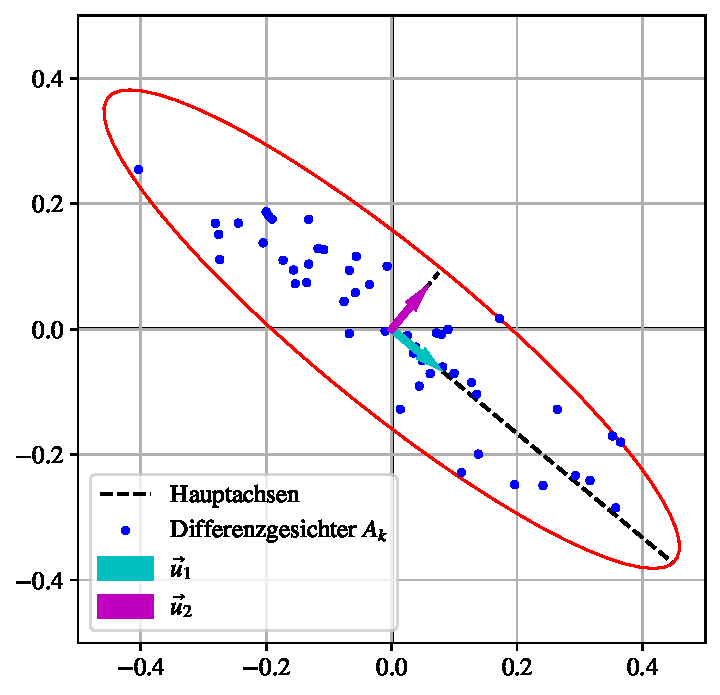
\includegraphics[width=0.45\textwidth]{images/facespace/principal_components} & 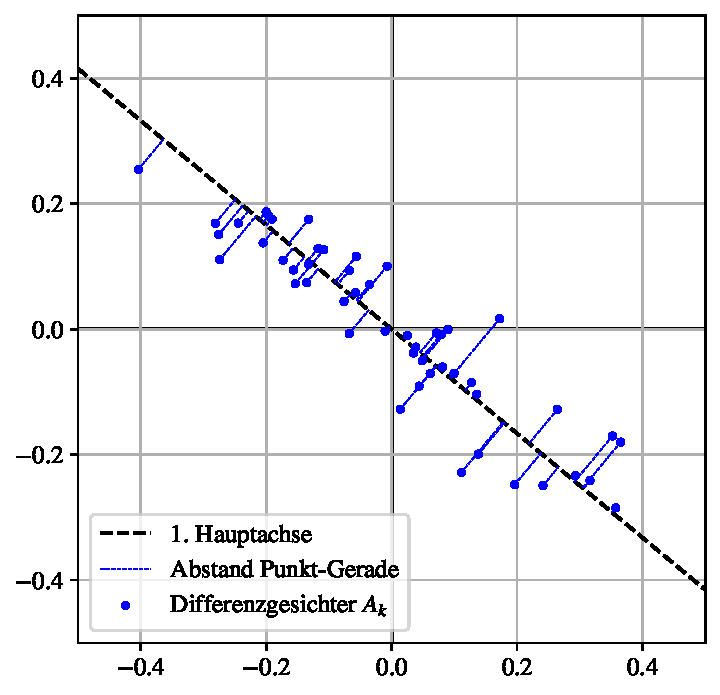
\includegraphics[width=0.45\textwidth]{images/facespace/distance_complicated} \\
	\end{tabular}
	\caption{Die Eigengesichter sind die orthonormalen Vektoren entlang den Hauptachsen. Die Eigengesichter $\vec u_1$ und $\vec u_2$ hätten eigentlich Länge 1, sind aber hier der Übersicht wegen zu kurz abgebildet.}
	\label{fig:construction}
\end{figure}

\begin{aufgabe} \label{aufg:eigenface_construction_0}
	Abbildung~\ref{fig:construction} zeig die Konstruktion nur in der Ebene und ist daher eine Vereinfachung.
	Nennen Sie zwei Unterschiede zwischen der Abbildung und unserer Situation.
	Nehmen Sie dabei an, dass wir Bilder der Auflösung $M\times N$ mit $M=180$ und $M=144$ betrachten.
\end{aufgabe}
\begin{losung}
	Die Abbildung entspricht dem Spezialfall $M\cdot N=2$.
	Im unserer Situation ist aber $M\cdot N=180\cdot 144=25920$.
	Das heisst, alle involvierten Vektoren haben 25920 Komponenten nur nicht nur 2.
	Zudem sind in der Abbildung nur zwei Eigengesichter $\vec u_1$ und $\vec u_2$ gezeigt, da es in der Ebene nicht mehr als zwei Vektoren geben kann, die alle paarweise orthogonal sind.
	In unserem Fall, also in einem Raum der Dimension 25920, kann es 25920 paarweise orthogonale Vektoren geben.
	Aber auch dann werden nur so viele Eigengesichter konstruiert, wie wir Gesichter in der Datenbank haben (deren Anzahl haben wir mit $K$ bezeichnet).
\end{losung}

\begin{aufgabe} \label{aufg:eigenface_construction_1}
	In der obigen Konstruktion der Eigengesichter muss man in jedem Schritt \glqq{}einen\grqq{} Vektor wählen, der folgende Bedingungen erfüllt:
	\begin{enumerate}[label=(\alph*)]
		\item \label{item:B1} Er hat Länge 1.
		\item \label{item:B2} Er ist orthogonal zu den bereits konstruierten Vektoren.
		\item\label{item:B3} Er zeigt in Richtung der grössten Streuung (unter allen Vektoren die Bedingung~\ref{item:B2} erfüllen).
	\end{enumerate}
	Warum das Wort \glqq{}einen\grqq{}?
	Gibt es denn Mehrere?
\end{aufgabe}
\begin{losung}
	Ja es gibt Mehrere.
	Immer wenn ein Vektor $\vec u$ die Bedingungen \ref{item:B1}, \ref{item:B2} und \ref{item:B3} erfüllt, so gilt das auch für $-\vec u$.
\end{losung}

Wir werden nun das erste Eigengesicht $\vec{u}_1$ berechnen.
Dazu müssen wir zuerst verstehen was es bedeutet, einen Vektor \glqq{}entlang der grössten Streuung\grqq{} zu finden.
Die erste Hauptachse wird wie folgt bestimmt:
Sie ist diejenige Gerade, welche die Summe der Abstandsquadrate zu den Punkten $A_1,\ldots,A_K$ minimiert.
Dies ist rechts in Abbildung~\ref{fig:construction} gezeigt.
Um die Eigengesichter zu berechnen, müssen wir also den Abstand eines Punktes von einer Geraden berechnen können.
\begin{aufgabe} \label{aufg:distance_simple}
	\begin{minipage}{0.55\textwidth}
		Berechnen Sie den Abstand des Punktes $A$ von der Geraden durch Null in Richtung $\vec{u}$, wobei $\vec{a}=\overrightarrow{OA}$ und
		\begin{align*}
			\vec{a}=
			\begin{pmatrix}
				1 \\
				-2
			\end{pmatrix},\quad
			\vec{u}=\frac{1}{5}
			\begin{pmatrix}
				4 \\
				-3
			\end{pmatrix}.
		\end{align*}
		\textit{Hinweis}: Der Vektor $\vec{u}$ hat Länge~1.
	\end{minipage}\hfill
	\begin{minipage}{0.4\textwidth}
		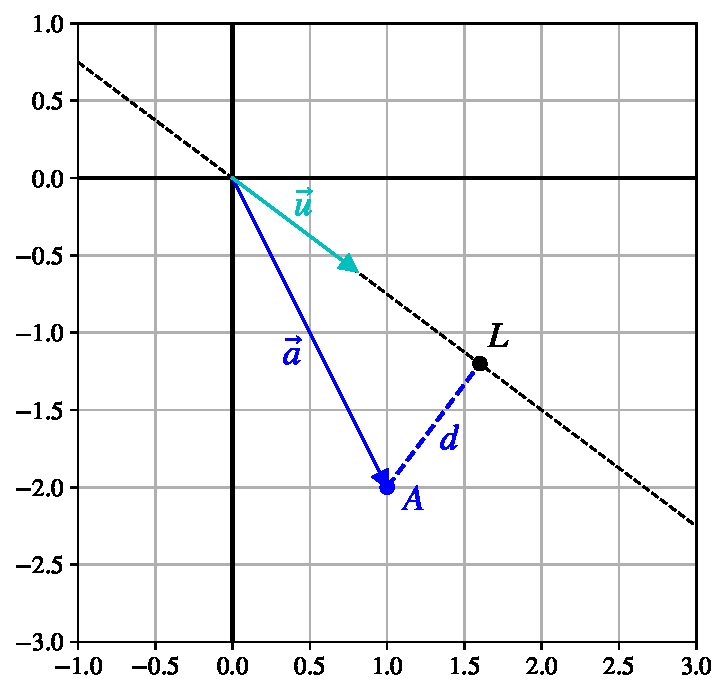
\includegraphics[width=\textwidth]{images/facespace/distance_simple}
	\end{minipage}
\end{aufgabe}
\begin{losung}
	Der Lotfusspunkt $L$ bezeichnet den Punkt auf der Geraden, welcher $A$ am nächsten liegt.
	Der Abstand von $L$ zum Ursprung ist $\vec{a}\cdot\vec{u}=2$.
	Dabei haben wir verwendet, dass $\vec{u}$ Länge 1 hat.
	Die gesuchte Distanz (blaue gestrichelte Linie im Bild) bezeichnen wir mit $d$.
	Nach dem Satz von Pythagoras gilt dann
	\begin{equation*}
		d^2+\left(\vec{a}\cdot\vec{u}\right)^2=\lVert\vec{a}\rVert^2.
	\end{equation*}
	Durch umformen erhalten wir
	\begin{equation*}
		d^2=\lVert\vec{a}\rVert^2-\left(\vec{a}\cdot\vec{u}\right)^2=5-4=1.
	\end{equation*}
	Der Abstand von $A$ zu Geraden ist also $d=1$.
\end{losung}
Was wir in Aufgabe~\ref{aufg:distance_simple} berechnet haben, funktioniert auch in höheren Dimensionen.
Seien $\vec v$ und $\vec w$ zwei Vektoren mit $M\cdot N$ Komponenten, also
\begin{equation*}
	\vec v=
	\begin{pmatrix}
		v_1 \\ v_2 \\ \vdots \\ v_{M\cdot N}
	\end{pmatrix},\qquad
	\vec w=
	\begin{pmatrix}
		w_1 \\ w_2 \\ \vdots \\ w_{M\cdot N}
	\end{pmatrix}.
\end{equation*}
Deren Skalarprodukt ist dann definiert als
\begin{equation*}
	\vec v\cdot\vec w=v_1w_1+\ldots+v_nw_n.
\end{equation*}
Ganz analog ist auch das Quadrat Länge eines Vektors gegeben durch $\lVert\vec v\rVert^2=\vec v\cdot\vec v$.
Der Abstand eines Punktes zu einer Geraden berechnet sich dann nach der selben Formel wie in der Lösung von Aufgabe~\ref{aufg:distance_simple}.
Das probieren wir zuerst für $M\cdot N=4$.
\begin{aufgabe} \label{aufg:distance_simple_1}
	Berechnen Sie den Abstand des Punktes $A$ von der Geraden durch Null in Richtung $\vec{u}$, wobei $\vec{a}=\overrightarrow{OA}$ und
	\begin{align*}
		\vec{a}=
		\begin{pmatrix}
			3 \\ -3 \\ 0 \\ 2
		\end{pmatrix},\quad
		\vec{u}=\frac{1}{2}
		\begin{pmatrix}
			1 \\ -1 \\ 1 \\ 1
		\end{pmatrix}.
	\end{align*}
	\textit{Hinweis}: Der Vektor $\vec{u}$ hat Länge~1.
\end{aufgabe}
\begin{losung}
	Obwohl wir es mit vierdimensionalen Vektoren zu tun haben, spielt sich das Problem noch immer in einer Ebene ab, nämlich der Ebene, die von $\vec a$ und $\vec u$ aufgespannt wird.
	Wir verfahren daher gleich wie in Aufgabe~\ref{aufg:distance_simple}.
	Der Abstand zum Lotfusspunkt $L$ ist gegeben durch
	\begin{equation*}
		\vec{a}\cdot\vec{u}=\tfrac{1}{2}\cdot 3+\left(-\tfrac{1}{2}\right)\cdot\left(-3\right)+\tfrac{1}{2}\cdot 0+\tfrac{1}{2}\cdot 2=4.
	\end{equation*}
	Dabei haben wir verwendet, dass $\vec{u}$ Länge 1 hat.
	Das Quadrat der Länge des Vektors $\vec a$ ist gegeben durch
	\begin{equation*}
		\lVert\vec{a}\rVert^2=\vec{a}\cdot\vec{a}=3^2+\left(-3\right)^2+0^2+2^2=22.
	\end{equation*}
	Die gesuchte Distanz bezeichnen wir mit $d$.
	Nach dem Satz von Pythagoras gilt dann
	\begin{equation*}
		d^2+\left(\vec{a}\cdot\vec{u}\right)^2=\lVert\vec{a}\rVert^2.
	\end{equation*}
	Durch umformen erhalten wir
	\begin{equation*}
		d^2=\lVert\vec{a}\rVert^2-\left(\vec{a}\cdot\vec{u}\right)^2=22-16=6.
	\end{equation*}
	Der Abstand von $A$ zu Geraden ist also $d=6$.
\end{losung}
\begin{aufgabe} \label{aufg:distance_complex}
	Sei $\vec{u}$ ein Vektor mit $M\cdot N$ Komponenten und Länge~1.
	Dieser definiert die Gerade durch Null in Richtung $\vec{u}$.
	Finden Sie eine Formel für die Summe der Abstandsquadrate aller Differenzgesichter $A_1,\ldots,A_K$ zu dieser Geraden.
	Dies ist rechts in Abbildung~\ref{fig:construction} dargestellt.
\end{aufgabe}
\begin{losung}
	Wir konzentrieren uns zuerst auf ein beliebiges Differenzgesicht $\vec{a}_k=\overrightarrow{OA_k}$, wobei $1\leq k\leq K$.
	Dessen Abstand zur Geraden bezeichnen wir mit $d_k$.
	Analog zu Aufgabe~\ref{aufg:distance_simple} gilt
	\begin{equation*}
		d_k^2=\lVert\vec{a}_k\rVert^2-\left(\vec{a}_k\cdot\vec{u}\right)^2.
	\end{equation*}
	Die Summe dieser Abstandsquadrate $d_1^2+\ldots+d_K^2$ ist demnach gegeben durch
	\begin{equation*}
		\lVert\vec{a}_1\rVert^2-\left(\vec{a}_1\cdot\vec{u}\right)^2
		+\lVert\vec{a}_2\rVert^2-\left(\vec{a}_2\cdot\vec{u}\right)^2
		+\ldots+
		\lVert\vec{a}_{M\cdot N}\rVert^2-\left(\vec{a}_{M\cdot N}\cdot\vec{u}\right)^2.
	\end{equation*}
\end{losung}
Die Formel aus Aufgabe~\ref{aufg:distance_complex} liefert für jedes $\vec{u}$ einen positiven Wert.
Dasjenige $\vec{u}$, welches diesen Ausdruck minimiert, ist das erste Eigengesicht $\vec{u}_1$.
Die Eigengesichter zu berechnen, heisst also ein Minimierungsproblem zu lösen.
Dies ist nicht so einfach und ist daher bereits implementiert.

Die Eigengesichter wollen wir nun visualisieren, indem wir sie wieder als Bilder darstellen.
Doch da gibt es noch ein Problem.
Die Komponenten der Eigengesichter liegen nicht notwendigerweise zwischen 0 und 1 und können daher nicht als Graustufen interpretiert werden.
Damit man sie als Bilder darstellen kann, müssen wir deren Komponenten zuerst in diese Teilmenge der reellen Zahl abbilden.
Dazu multipliziert man jedes Eigengesicht mit einem gewissen Faktor, welcher vom Mass der Streuung entlang dieses Eigengesichtes abhängt.
Dann entspricht das Eigengesicht ungefähr einem Differenzgesicht, welches man wieder durch Addition von $\vec m$ zu einem Vektor mit Einträgen zwischen 0 und 1 verschieben kann.
Wir wollen hier nicht genauer darauf eingehen.
Der Vollständigkeit halber geben wir aber in Abbildung~\ref{fig:eigenfaces} das Resultat an.
\begin{figure}[ht]
	\begin{tabular}{cccccccc}
		\includegraphics[width=0.1\textwidth]{images/eigenfaces/eigenface00} & \includegraphics[width=0.1\textwidth]{images/eigenfaces/eigenface01} &
		\includegraphics[width=0.1\textwidth]{images/eigenfaces/eigenface02} & \includegraphics[width=0.1\textwidth]{images/eigenfaces/eigenface03} &
		\includegraphics[width=0.1\textwidth]{images/eigenfaces/eigenface04} &
		\includegraphics[width=0.1\textwidth]{images/eigenfaces/eigenface05} & \includegraphics[width=0.1\textwidth]{images/eigenfaces/eigenface06} &
		\includegraphics[width=0.1\textwidth]{images/eigenfaces/eigenface07} \\ \includegraphics[width=0.1\textwidth]{images/eigenfaces/eigenface08} &
		\includegraphics[width=0.1\textwidth]{images/eigenfaces/eigenface09} & \includegraphics[width=0.1\textwidth]{images/eigenfaces/eigenface10} &
		\includegraphics[width=0.1\textwidth]{images/eigenfaces/eigenface11} & \includegraphics[width=0.1\textwidth]{images/eigenfaces/eigenface12} &
		\includegraphics[width=0.1\textwidth]{images/eigenfaces/eigenface13} & \includegraphics[width=0.1\textwidth]{images/eigenfaces/eigenface14} &
		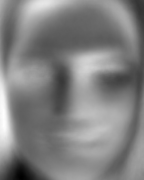
\includegraphics[width=0.1\textwidth]{images/eigenfaces/eigenface15} \\
	\end{tabular}
	\captionof{figure}{Die ersten 16 Eigengesichter wurden wieder als Bild dargestellt.}
	\label{fig:eigenfaces}
\end{figure}

Im Grunde fangen die Eigengesichter charakteristische Gesichtszüge ein.
Mit charakteristisch ist hier gemeint, dass genau diese Gesichtszüge für die grösste Streuung unter allen Bildern der Datenbank verantwortlich sind.
Sie beschreiben die Merkmale, nach denen sich die Gesichter am meisten unterscheiden.
Besser gesagt: Das erste Eigengesicht fängt den Gesichtszug mit der grössten Streuung ein.
Die weiteren Eigengesichter fangen Gesichtszüge mit immer weniger Streuung ein.
Dies spiegelt sich auch in deren Konstruktion wieder, welche die Eigengesichter ja gerade als Vektoren entlang der grössten Streuung definiert.

%Das machen wir wie folgt:
%Sei $\vec v$ ein Vektor mit $M\cdot N$ Komponenten, welche nicht notwendigerweise zwischen 0 und 1 liegen.
%Sei $\min\left(\vec v\right)$ das Minimum und $\max\left(\vec v\right)$ das Maximum aller Komponenten von $\vec v$.
%Wir betrachten nun den Vektor
%\begin{equation*}
%	\vec w=
%	\begin{pmatrix}
%		w_1 \\
%		w_2 \\
%		\vdots \\
%		w_{M\cdot N}
%	\end{pmatrix}
%\end{equation*}
%dessen Komponenten sich aus denen von $\vec v$ wie folgt zusammensetzen
%\begin{equation*}
%	w_i=\frac{v_i-\min\left(\vec v\right)}{\max\left(\vec v\right)-\min\left(\vec v\right)},
%	\qquad i=1,\ldots,M\cdot N.
%\end{equation*}
%Die Komponenten des Vektors $\vec w$ liegen dann alle in zwischen 0 und 1.
%Falls alle Komponenten von $\vec v$ gleich sind, ist $\min\left(\vec v\right)=\max\left(\vec v\right)$ und wir haben eine Division durch Null.
%Wir ignorieren diesen Fall.
%\begin{aufgabe} \label{aufg:scaling_theory}
%	\begin{enumerate}[label=(\alph*)]
%		\item Betrachten Sie den Vektor
%		\begin{equation*}
%			\vec v=
%			\begin{pmatrix}
%				-2 \\
%				4 \\
%				1
%			\end{pmatrix}.
%		\end{equation*}
%		Berechnen Sie daraus den Vektor $\vec w$ gemäss obigem Verfahren.
%		\item Begründen Sie, warum dieses Verfahren immer einen Vektor mit Komponenten zwischen 0 und 1 liefert, auch für einen allgemeinen Vektor $\vec v$.
%	\end{enumerate}
%\end{aufgabe}
%\begin{losung}
%	\begin{enumerate}[label=(\alph*)]
%		\item In obigem Beispiel ist $\min\left(\vec v\right)=-2$ und $\max\left(\vec v\right)=4$.
%		Daraus ergibt sich für alle $i\in\left\{1,2,3\right\}$
%		\begin{equation*}
%			w_i=\frac{v_i-\left(-2\right)}{4-\left(-2\right)}=\frac{v_i+2}{6}.
%		\end{equation*}
%		Somit erhalten wir
%		\begin{equation*}
%			\vec w=
%			\begin{pmatrix}
%				0 \\
%				1 \\
%				\tfrac{1}{2}
%			\end{pmatrix}.
%		\end{equation*}
%		\item Für alle Komponenten $v_i$ gilt stets
%		\begin{equation*}
%			\min\left(\vec v\right)\leq v_i\leq\max\left(\vec v\right).
%		\end{equation*}
%		Daraus folgt, dass im Bruch
%		\begin{equation*}
%			w_i=\frac{v_i-\min\left(\vec v\right)}{\max\left(\vec v\right)-\min\left(\vec v\right)},
%		\end{equation*}
%		der Nenner immer grösser oder Gleich dem Zähler ist, und dass beide nicht negativ werden können.
%		Folglich muss $0\leq w_i\leq 1$ gelten.
%	\end{enumerate}
%\end{losung}
%\begin{aufgabe} \label{aufg:scaling_code}
%	Ergänzen Sie die Funktion \texttt{interpolate(v)}, welche den Vektor mit Komponenten in zwischen 0 und 1 zurück gibt, der aus dem Vektor \texttt{v} durch obiges Verfahren entsteht.
%	Testen Sie ihre Lösung mit dem Python Skript \texttt{plot\_eigenfaces.py}, welches ihre Funktion \texttt{interpolate(v)} auf die Eigengesichter $\vec u_1,\ldots,\vec u_K$ anwendet und diese als Bilder abspeichert.
%	\textit{Hinweis:} Die Funktionen \texttt{np.min(v)} und \texttt{np.max(v)} liefern das Minimum und das Maximum eines Vektors \texttt{v}.
%\end{aufgabe}
%\begin{losung}
%	Eine mögliche Lösung ist unten gezeigt.
%	Die Eigengesichter sind in Abbildung~\ref{fig:eigenfaces} dargestellt.
%\begin{lstlisting}[style=python]
%import numpy as np
%
%def interpolate(v):
%	MN = len(v)
%	w = np.zeros_like(v)
%	a = np.min(v)
%	b = np.max(v)
%	for i in range(MN):
%		w[i] = (v[i] - a) / (b - a)
%	return w
%\end{lstlisting}
%\begin{center}
%	\begin{tabular}{cccccccc}
%		\includegraphics[width=0.1\textwidth]{images/eigenfaces/eigenface00} & \includegraphics[width=0.1\textwidth]{images/eigenfaces/eigenface01} &
%		\includegraphics[width=0.1\textwidth]{images/eigenfaces/eigenface02} & \includegraphics[width=0.1\textwidth]{images/eigenfaces/eigenface03} &
%		\includegraphics[width=0.1\textwidth]{images/eigenfaces/eigenface04} &
%		\includegraphics[width=0.1\textwidth]{images/eigenfaces/eigenface05} & \includegraphics[width=0.1\textwidth]{images/eigenfaces/eigenface06} &
%		\includegraphics[width=0.1\textwidth]{images/eigenfaces/eigenface07} \\ \includegraphics[width=0.1\textwidth]{images/eigenfaces/eigenface08} &
%		\includegraphics[width=0.1\textwidth]{images/eigenfaces/eigenface09} & \includegraphics[width=0.1\textwidth]{images/eigenfaces/eigenface10} &
%		\includegraphics[width=0.1\textwidth]{images/eigenfaces/eigenface11} & \includegraphics[width=0.1\textwidth]{images/eigenfaces/eigenface12} &
%		\includegraphics[width=0.1\textwidth]{images/eigenfaces/eigenface13} & \includegraphics[width=0.1\textwidth]{images/eigenfaces/eigenface14} &
%		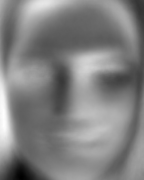
\includegraphics[width=0.1\textwidth]{images/eigenfaces/eigenface15} \\
%	\end{tabular}
%	\captionof{figure}{Die ersten 16 Eigengesichter wurden wieder als Bild dargestellt.}
%	\label{fig:eigenfaces}
%\end{center}
%\end{losung}
%
%Im Grunde fangen die Eigengesichter charakteristische Gesichtszüge ein.
%Mit charakteristisch ist hier gemeint, dass genau diese Gesichtszüge für die grösste Streuung unter allen Bildern der Datenbank verantwortlich sind.
%Sie beschreiben die Merkmale, nach denen sich die Gesichter am meisten unterscheiden.
%Besser gesagt: Das erste Eigengesicht fängt den Gesichtszug mit der grössten Streuung ein.
%Die weiteren Eigengesichter fangen Gesichtszüge mit immer weniger Streuung ein.
%Dies spiegelt sich auch in deren Konstruktion wieder, welche die Eigengesichter ja gerade als Vektoren entlang der grössten Streuung definiert.
%
%Tatsächlich kann man das Mass dieser Streuung (die sogenannte Varianz) nutzen, um die Eigengesichter auf bessere Weise in Bilder umzuwandeln, als wir es in Aufgabe~\ref{aufg:scaling_code} getan haben.
%Wir wollen hier weder darauf eingehen, was \glqq{}besser\grqq{} heisst, noch wie man das genau berechnen kann.
%Der Vollständigkeit halber geben wir aber in Abbildung~\ref{fig:eigenfaces_best} das Resultat an.
%\begin{figure}[ht]
%	\begin{tabular}{cccccccc}
%		\includegraphics[width=0.1\textwidth]{images/eigenfaces_best/eigenface00} & \includegraphics[width=0.1\textwidth]{images/eigenfaces_best/eigenface01} &
%		\includegraphics[width=0.1\textwidth]{images/eigenfaces_best/eigenface02} & \includegraphics[width=0.1\textwidth]{images/eigenfaces_best/eigenface03} &
%		\includegraphics[width=0.1\textwidth]{images/eigenfaces_best/eigenface04} &
%		\includegraphics[width=0.1\textwidth]{images/eigenfaces_best/eigenface05} & \includegraphics[width=0.1\textwidth]{images/eigenfaces_best/eigenface06} &
%		\includegraphics[width=0.1\textwidth]{images/eigenfaces_best/eigenface07} \\ \includegraphics[width=0.1\textwidth]{images/eigenfaces_best/eigenface08} &
%		\includegraphics[width=0.1\textwidth]{images/eigenfaces_best/eigenface09} & \includegraphics[width=0.1\textwidth]{images/eigenfaces_best/eigenface10} &
%		\includegraphics[width=0.1\textwidth]{images/eigenfaces_best/eigenface11} & \includegraphics[width=0.1\textwidth]{images/eigenfaces_best/eigenface12} &
%		\includegraphics[width=0.1\textwidth]{images/eigenfaces_best/eigenface13} & \includegraphics[width=0.1\textwidth]{images/eigenfaces_best/eigenface14} &
%		\includegraphics[width=0.1\textwidth]{images/eigenfaces_best/eigenface15} \\
%	\end{tabular}
%	\captionof{figure}{Die ersten 16 Eigengesichter wurden wieder als Bild dargestellt. Man vergleiche mit Abbildung~\ref{fig:eigenfaces}.}
%	\label{fig:eigenfaces_best}
%\end{figure}